\documentclass{article}

\title{Práctica 3 de Criptografía y Computación}
\date{}
\author{Carlos Núñez Molina \\ Alessandro Zito \\ Gabriela Antolinez}

\usepackage{titlesec}
\usepackage{graphicx}



\titleformat{\section}
  {\normalfont\large}{\thesection}{1em}{}

\begin{document}
	\maketitle
	\newpage





    \section{Análisis tiempos Factorización}

    En esta sección vamos a analizar como tarda el algoritmo de Factorizacion por números grandes. Utilizaremos los tres metodologías que tiene ese algoritmo: Fuerza Bruta, Fermat y Ro de Pollard. Hemos hecho los análisis de frecuencias con números al azar y con números productos de primos. Empezaremos comentando con los números al azar. Hemos factorizando los números completamente (no encontramos un solo factor sino todos los factores), y vamos analizando cómo varía la eficiencia de los algoritmos según aumenta el número de cifras (en formato decimal, no binario). Además, hemos hecho experimentos para dos tipos de números: aquellos elegidos al azar y aquellos que son producto de dos primos de forma que el número resultante tiene n cifras.


    Empezando con el algoritmo de Fuerza Bruta, sabemos que este algoritmo va intentando hasta que no factoriza el numero. Podemos ver en la primera imagen, El algoritmo es capaz de factorizar números de hastas 28 cifras, a partir de los cuales ya tarda demasiado. Su eficiencia es exponencial en el número de cifras, llegando a tardar \begin{math} 10^{2} \end{math} segundos cuando el número tiene 28 cifras." de \begin{math} 10^{2} \end{math}



    \begin{figure}[ht!]
        \centering
        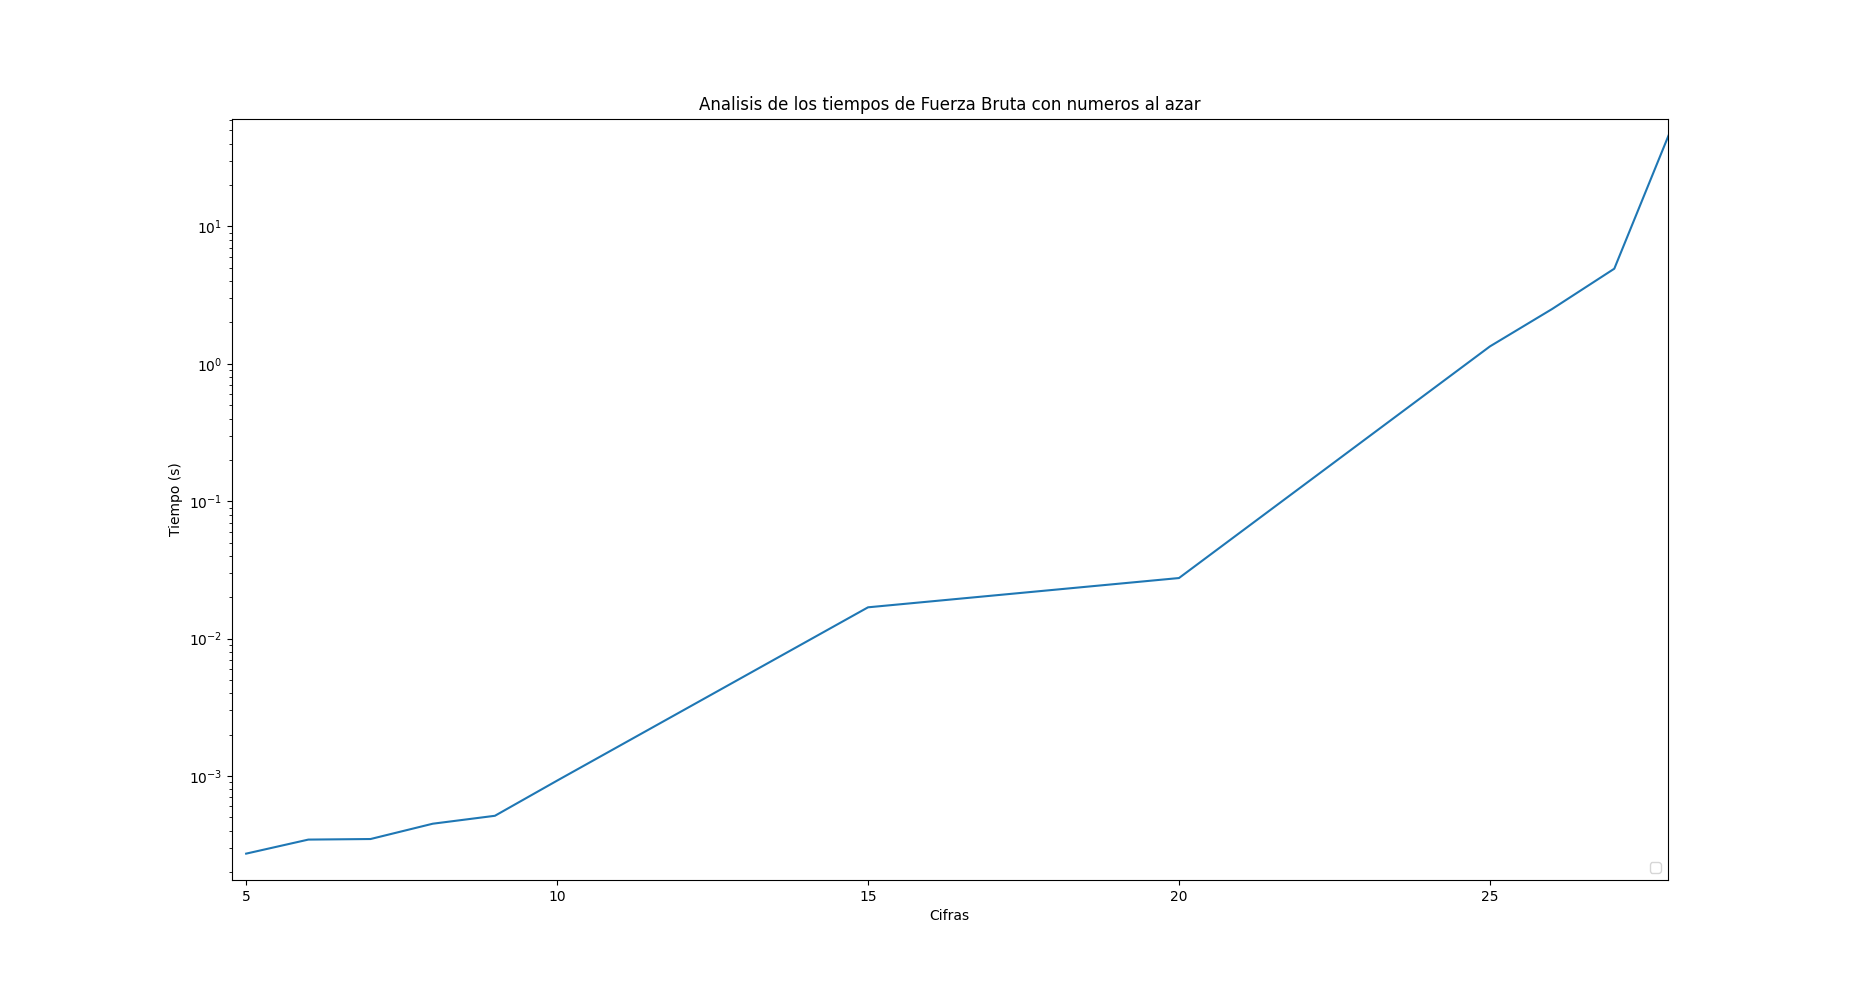
\includegraphics[scale=0.3]{Figure_1}
        \caption{Análisis de los tiempos de Fuerza Bruta con números al azar}
        \label{fig:Figure_1}
    \end{figure}

    \newpage

     Después siguiendo con el algoritmo de Fermat, sabemos que este algoritmo va a resolver la ecuación \begin{math} y = x ^{2} - n \end{math} para factorizar el numero. Podemos ver en la imagen que este algoritmo es el peor de los tres, ya que solo es capaz de factorizar en un tiempo razonable números de hasta 10 cifras. El algoritmo es el peor de los tres por cómo factoriza los números: intenta factorizar el número de la forma \begin{math} (x-n)*(x+n)\end{math}. Así, estos dos factores tienen que estar próximos entre sí (y de la raíz cuadrada del número a factorizar) para que el método funcione bien (si no lo están, tarda mucho). En los números elegidos al azar esto no pasa, ya que suelen tener divisores pequeños, y por eso funciona tan mal.



    \begin{figure}[ht!]
        \centering
        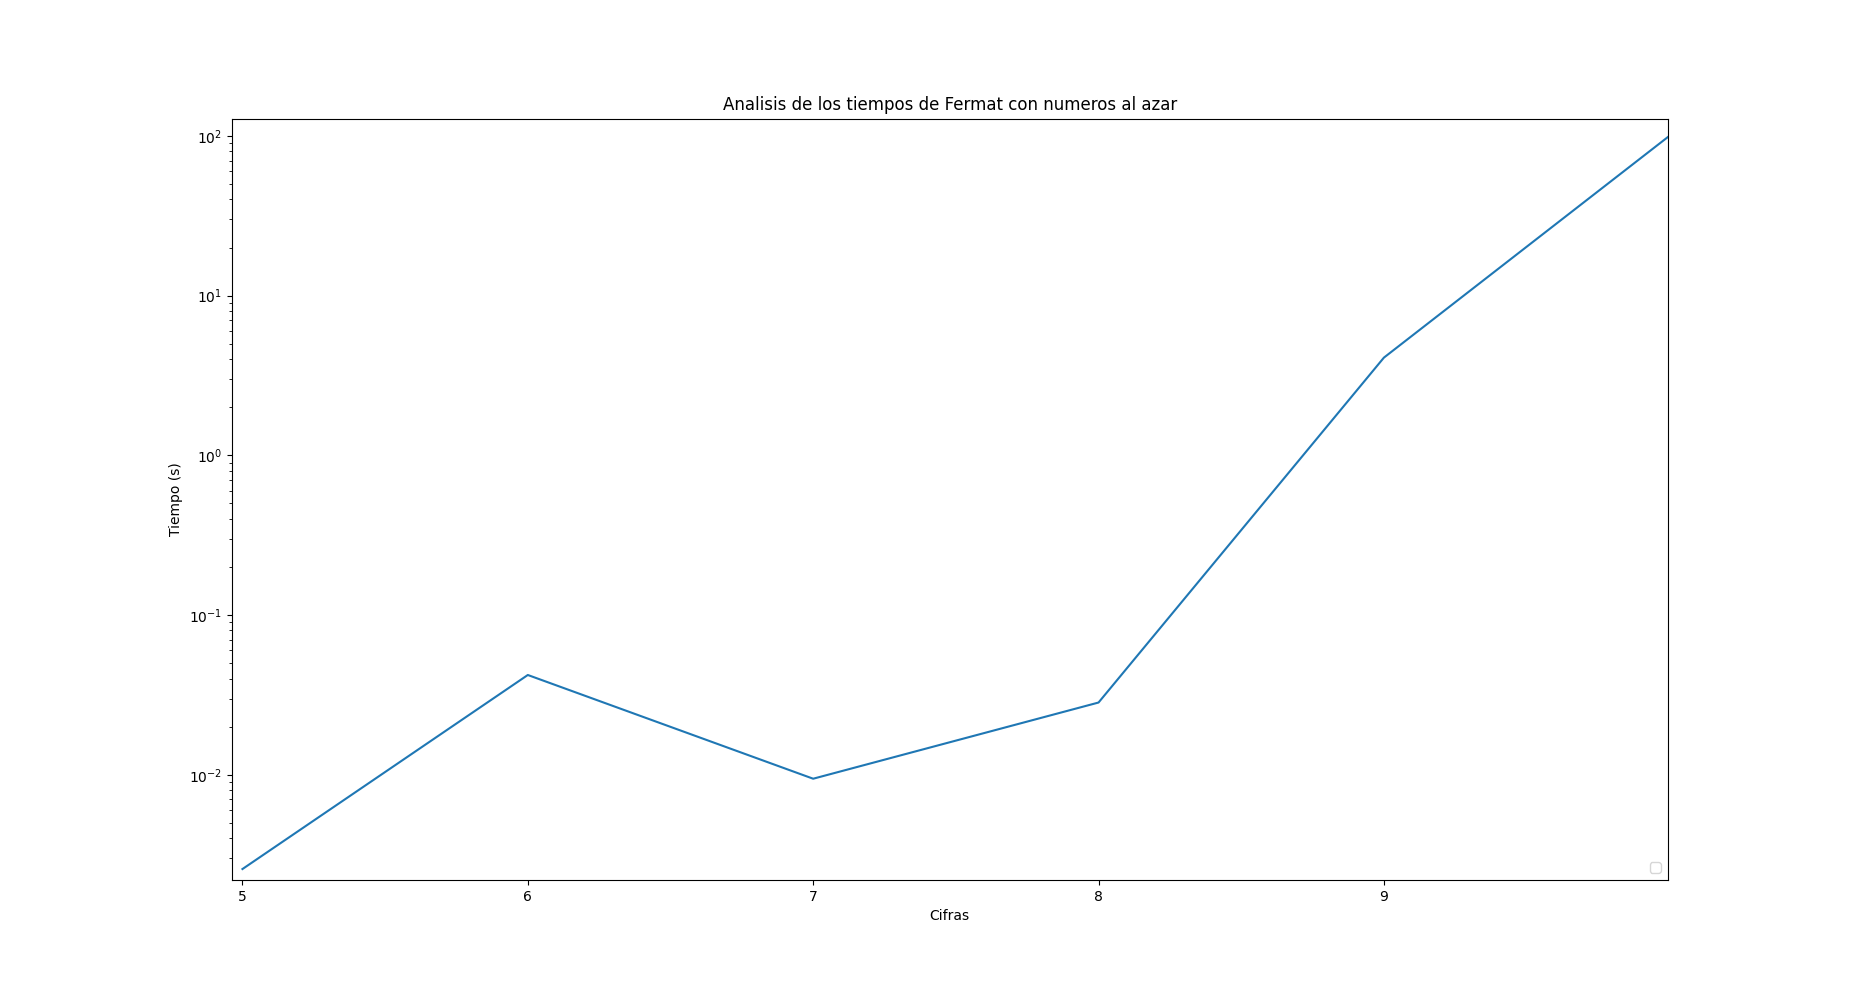
\includegraphics[scale=0.3]{Figure_3}
        \caption{Análisis de los tiempos de Fermat con números al azar}
        \label{fig:Figure_3}
    \end{figure}

    \newpage


    El ultimo de los tres el algoritmo de Ro de Pollard, que tiene el nombre de el matemático que lo inventó. Se trata de construir una sucesión
    \begin{math} x_{1}, x_{2}, ..., x_{n} \end{math} y encontrar dos términos de la sucesión
    \begin{math}  x_{i}, x_{j} \end{math} tales que \begin{math} mcd(x_{i} - x_{j} ; n) \neq 1. \end{math} Podemos ver que este algoritmo es el mas eficiente de los 3, porqué se tardará "solo" 100 segundos con numerosa de 42 cifras!


    \begin{figure}[ht!]
        \centering
        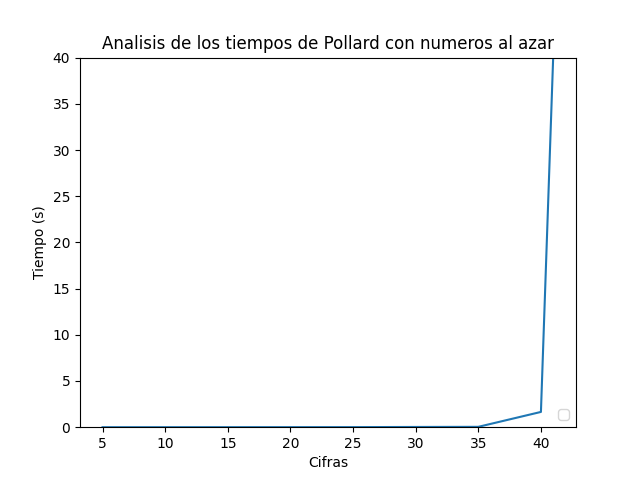
\includegraphics[scale=0.3]{Figure_5}
        \caption{Análisis de los tiempos de Pollard con números al azar}
        \label{fig:Figure_5}
    \end{figure}


    \newpage


    Haciendo los mismos test con números productos de dos primos, podemos ver como Fuerza  bruta y pollard tardan más porque los números son más difíciles de factorizar: tienen solo dos factores y son más grandes que cuando los números se eligen al azar. Sin embargo, fermat tarda menos con este tipo de números porque ambos factores están más cerca entre sí y de la raíz cuadrada del número. El mejor sigue siendo pollard que factoriza hasta las 28 cifras, pero que ahora fuerza bruta y fermat son más o menos igual de eficientes, aunque fuerza bruta sigue siendo mejor que fermat factorizando 20 cifrad y fermat 18 cifras

    \begin{figure}[ht!]
        \centering
        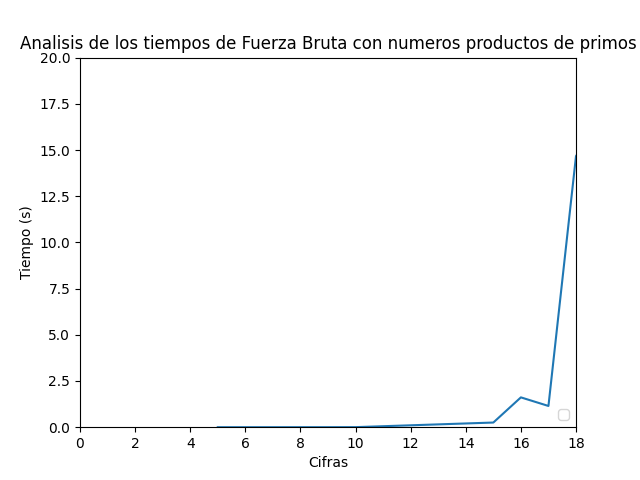
\includegraphics[scale=0.3]{Figure_2}
        \caption{Análisis de los tiempos de Fuerza Bruta con números productos de dos primos}
        \label{fig:Figure_2}
    \end{figure}

    \begin{figure}[ht!]
        \centering
        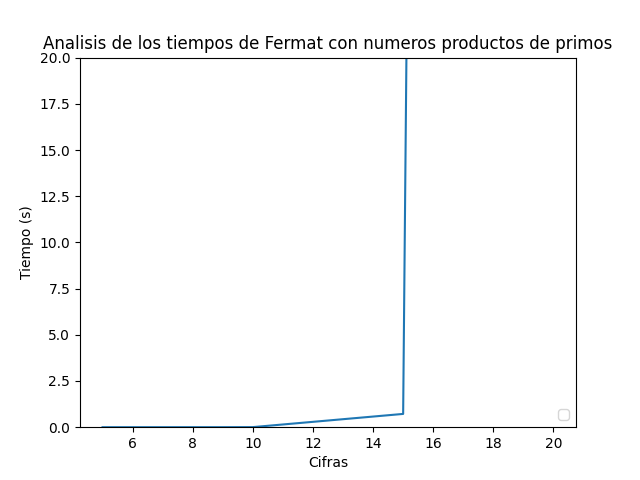
\includegraphics[scale=0.3]{Figure_4}
        \caption{Análisis de los tiempos de Fermat con números productos de dos primos}
        \label{fig:Figure_4}
    \end{figure}

    \begin{figure}[ht!]
        \centering
        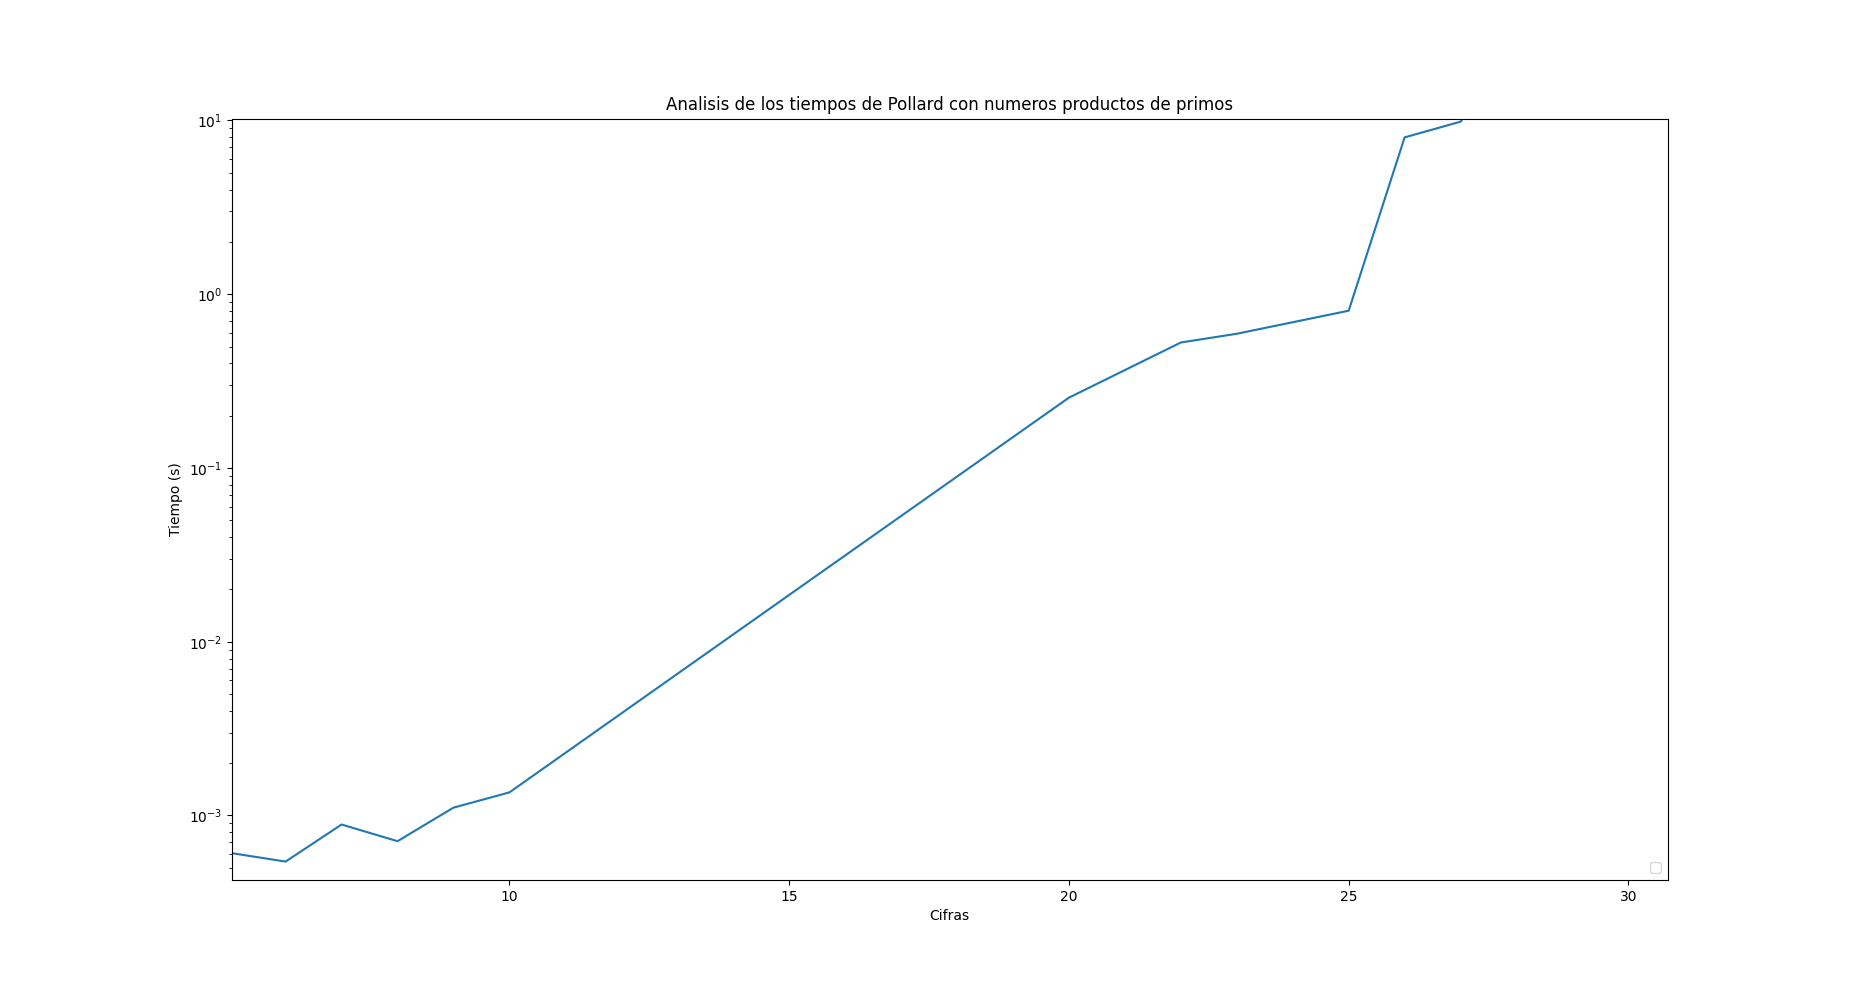
\includegraphics[scale=0.3]{Figure_6}
        \caption{Análisis de los tiempos de Pollard con números productos de dos primos}
        \label{fig:Figure_6}
    \end{figure}

    \newpage


    \section{Estimaciones}
    Hemos hecho una  estimación para ver cuanto tardaba cada algoritmo con un numero de 50 cifras. Lo que hemos hecho es estimar simplemente hemos dividido el tiempo para cada número de cifras entre el tiempo anterior y después hemos hecho la media. Después hemos encontrado cuánto aumenta de media el tiempo cuando se aumenta el número de cifras en 1 y hemos usado eso para estimar el tiempo para 50 cifras (no hemos usado los tiempos pequeños porque al ser tan pequeños son imprecisos).
    Lo resultados son:
    \begin{itemize}
        \item Fuerza Bruta:
        \begin{itemize}
            \item Número de 50 cifras al azar: 1.394766457605177e+34
            \item Número de 50 cifras producto de primos: 2.1029773066486474e+80
        \end{itemize}
        \item Fermat:
        \begin{itemize}
            \item Número de 50 cifras al azar: 2.2167256626584056e+68
            \item Número de 50 cifras producto de primos: 4.378776394397684e+74
        \end{itemize}
        \item Ro de Pollard:
        \begin{itemize}
            \item Número de 50 cifras al azar: 5.995733542705329e+30
            \item Número de 50 cifras producto de primos: 2.9305515186779655e+20
        \end{itemize}
    \end{itemize}

    Como se puede ver, Pollard tarda meno en calcular el numero en ambo los metodos; Fermat tarda meno que Fuerza Bruta en numero producto de primos pero sigue siendo el peor de los tres.

    \newpage

    \section{Conclusiones}

    A partir de esos resultados lo único que sacamos es que cualquiera de los algoritmos no son capaces de factorizar números de 50 cifras (incluso el mejor de ellos tardaría billones de años). Como se puede ver, Pollard tarda meno en calcular el numero en ambo los metodos; Fermat tarda meno que Fuerza Bruta en numero producto de primos pero sigue siendo el peor de los tres.

    \newblock
    Creemos que el peor de los tres métodos es fermat: funciona peor que fuerza bruta para números al azar y cuando son producto de primos funciona mejor pero sigue siendo peor que fuerza bruta. El mejor de los tres métodos es pollard, ya que es el mejor sin importar si los números son escogidos al azar o producto de primos.



\end{document}